
\documentclass[tikz,border=5pt]{standalone}
\usepackage[T1]{fontenc}
\usepackage{newtxtext,newtxmath}
\usepackage{tikz}
\usetikzlibrary{arrows.meta,positioning,fit,calc}
\definecolor{oasiblue}{RGB}{45,82,122}
\definecolor{oasigreen}{RGB}{63,108,79}
\definecolor{oasiorange}{RGB}{150,92,40}
\definecolor{oasired}{RGB}{132,54,54}
\definecolor{oasigray}{RGB}{84,91,99}
\begin{document}
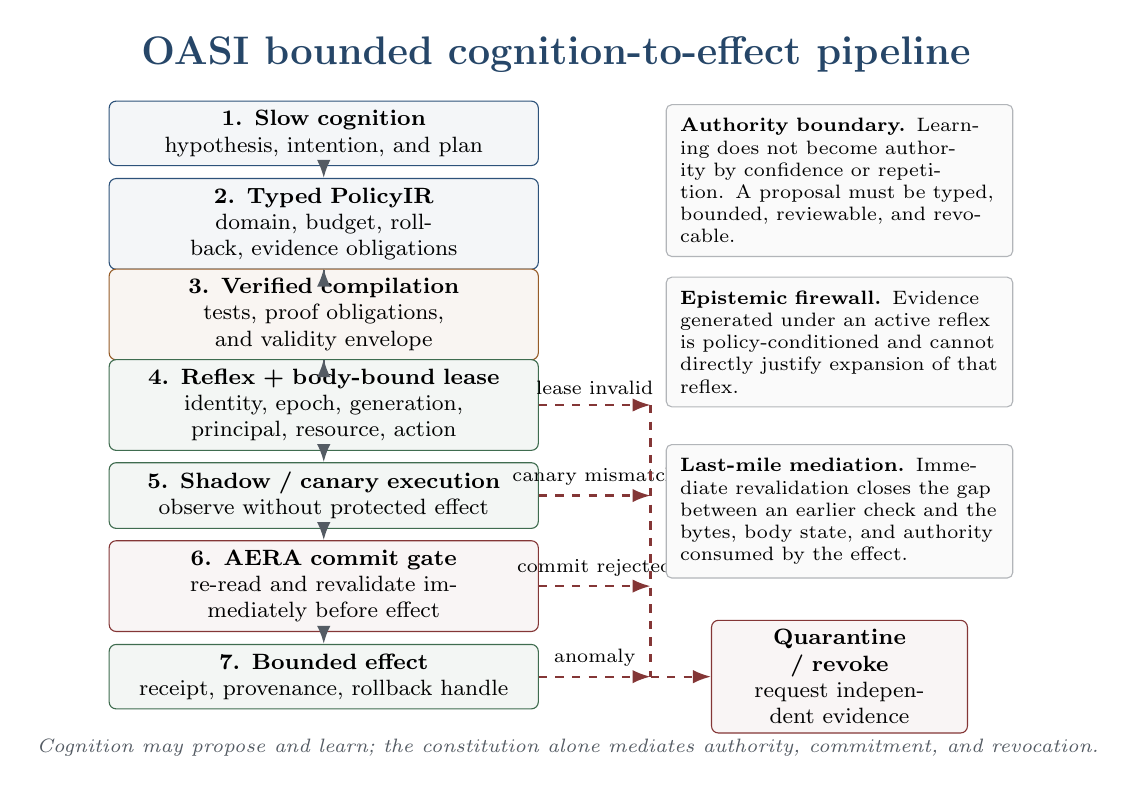
\begin{tikzpicture}[
  font=\footnotesize, >=Latex,
  stage/.style={draw,rounded corners=2.5pt,minimum width=5.45cm,text width=5.05cm,
    minimum height=.78cm,align=center,fill=white},
  blue/.style={stage,draw=oasiblue,fill=oasiblue!5},
  green/.style={stage,draw=oasigreen,fill=oasigreen!6},
  orange/.style={stage,draw=oasiorange,fill=oasiorange!6},
  red/.style={stage,draw=oasired,fill=oasired!5},
  arr/.style={->,line width=.78pt,draw=oasigray},
  ex/.style={->,dashed,line width=.78pt,draw=oasired},
  note/.style={draw=oasigray!45,rounded corners=2pt,fill=oasigray!3,
    text width=4.05cm,align=left,font=\scriptsize,inner sep=5pt}
]
\node[font=\bfseries\Large,text=oasiblue!85!black] at (2.95,4.25)
 {OASI bounded cognition-to-effect pipeline};

\node[blue] (s1) at (0,3.25) {\textbf{1. Slow cognition}\\hypothesis, intention, and plan};
\node[blue] (s2) at (0,2.10) {\textbf{2. Typed PolicyIR}\\domain, budget, rollback, evidence obligations};
\node[orange] (s3) at (0,.95) {\textbf{3. Verified compilation}\\tests, proof obligations, and validity envelope};
\node[green] (s4) at (0,-.20) {\textbf{4. Reflex + body-bound lease}\\identity, epoch, generation, principal, resource, action};
\node[green] (s5) at (0,-1.35) {\textbf{5. Shadow / canary execution}\\observe without protected effect};
\node[red] (s6) at (0,-2.50) {\textbf{6. AERA commit gate}\\re-read and revalidate immediately before effect};
\node[green] (s7) at (0,-3.65) {\textbf{7. Bounded effect}\\receipt, provenance, rollback handle};

\draw[arr] (s1) -- (s2);
\draw[arr] (s2) -- (s3);
\draw[arr] (s3) -- (s4);
\draw[arr] (s4) -- (s5);
\draw[arr] (s5) -- (s6);
\draw[arr] (s6) -- (s7);

\coordinate (busTop) at (4.15,-.20);
\coordinate (busMid) at (4.15,-1.35);
\coordinate (busLow) at (4.15,-2.50);
\coordinate (busBottom) at (4.15,-3.65);
\draw[ex] (s4.east) -- node[above,font=\scriptsize]{lease invalid} (busTop);
\draw[ex] (s5.east) -- node[above,font=\scriptsize]{canary mismatch} (busMid);
\draw[ex] (s6.east) -- node[above,font=\scriptsize]{commit rejected} (busLow);
\draw[ex] (s7.east) -- node[above,font=\scriptsize]{anomaly} (busBottom);
\draw[draw=oasired,dashed,line width=.78pt] (busTop) -- (busBottom);

\node[red,minimum width=3.25cm,text width=2.95cm] (q) at (6.55,-3.65)
 {\textbf{Quarantine / revoke}\\request independent evidence};
\draw[ex] (busBottom) -- (q.west);

\node[note] at (6.55,2.65)
 {\textbf{Authority boundary.} Learning does not become authority by confidence or repetition. A proposal must be typed, bounded, reviewable, and revocable.};
\node[note] at (6.55,.60)
 {\textbf{Epistemic firewall.} Evidence generated under an active reflex is policy-conditioned and cannot directly justify expansion of that reflex.};
\node[note] at (6.55,-1.55)
 {\textbf{Last-mile mediation.} Immediate revalidation closes the gap between an earlier check and the bytes, body state, and authority consumed by the effect.};

\node[font=\itshape\scriptsize,text=oasigray,align=center] at (3.1,-4.55)
 {Cognition may propose and learn; the constitution alone mediates authority, commitment, and revocation.};
\end{tikzpicture}
\end{document}
